\documentclass{assignment}
\usepackage{amsmath}
\usepackage{lipsum}
\usepackage{multicol}
\usepackage{fancyhdr}
\usepackage{graphicx}
\usepackage{blindtext}
\usepackage[dvipsnames]{xcolor}
\usepackage{enumitem}
\usepackage{cleveref}
\usepackage{color,soul}
\usepackage{amsfonts}
\def\code#1{\texttt{#1}}
\newtheorem{anm}{Anm}

\begin{document}


\assignmentTitle
{n/a}{n/a}
{n/a}
{n/a}
{assets/KTH_logga.png}
{Partikel}
{Projekt}

\section{Introduction}

Vi betraktar en modell av en tvättmaskin enligt angiven figur. 
Det finns en klump med våta kläder med massan $m$ inuti maskinen som skapar en obalans när maskinen roterar. 
Massan av maskinens roterande del utan kläder är $M$ och lasttrummans radie är $r$. 
Rotationsdelens rörelse styrs och dämpas av ett system som kan modelleras med fjädrar och dämpare enligt figuren, där $k$ och $c$ är fjäderkonstanten respektive dämpningskonstanten.

\section{Friläggning}
\begin{figure}[!h]
    \centering
    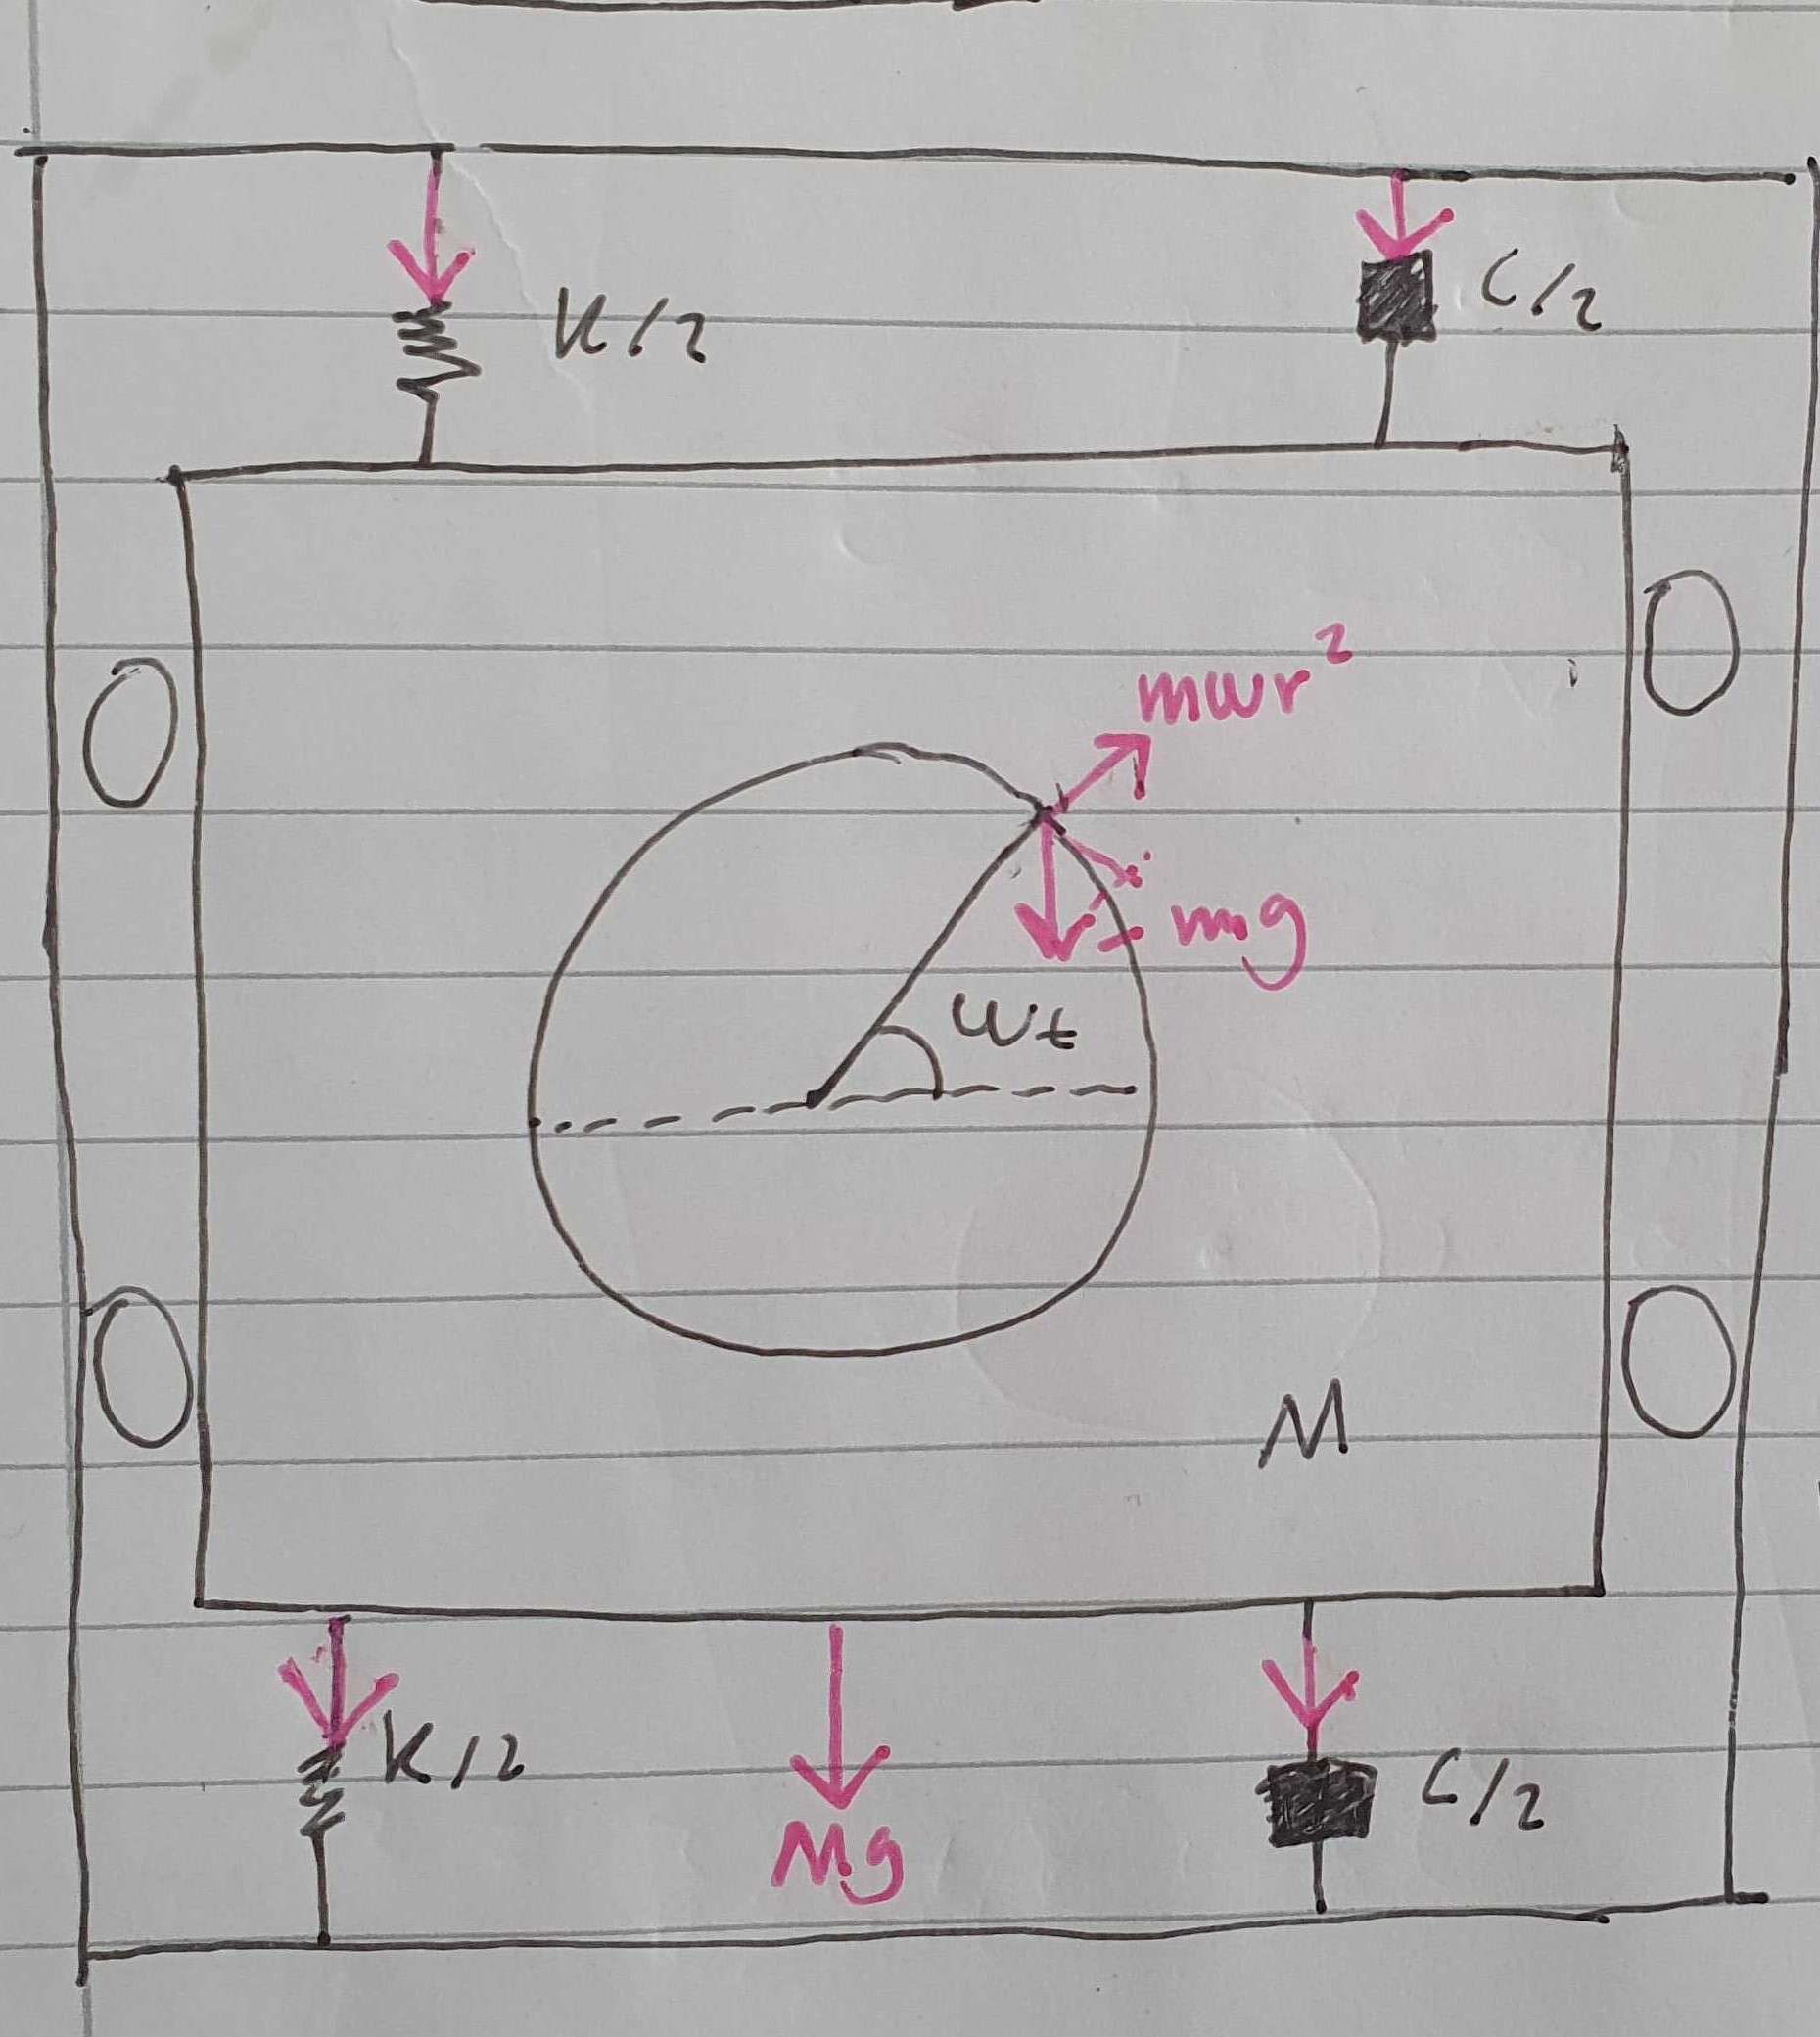
\includegraphics[width = 70mm]{assets/diagram.jpg}
    \caption{Caption}
    \label{fig:my_label}
\end{figure}

\newpage
\section{Kraftekvationer för den fria delen}
Vi har att 
\begin{align}
    M \frac{d^2 y}{d t^2}+m \frac{d^2}{d t^2}(y+r \sin \omega t)=-k y-c \frac{d y}{d t}
\end{align}
där $M$ och $m$ är massorna för den ickeroterande delen respektive roterande delen av tvättmaskinen.
Efter förkortning får vi följande svägningsekvation;

\begin{align}
\ddot{y}+\frac{c \dot{y}}{M+m}+\frac{k y}{M+m}=\frac{m}{M+m} r \cdot w^2 \sin (wt)
\end{align}

Detta ger $2\zeta \omega_n=\frac{c}{M+m}$ och $\omega_n^2=\frac{k}{M+m}$
vilket slutligen ger oss 
\begin{align}
    \ddot{y}+2 \zeta \omega_n \dot{y}+\omega_n^2 y=\frac{m}{M+m} r\omega^2 \sin \omega t
\end{align}
Ekvationen är en icke-homogen, vi har därför en lösning på formen 
$r(t)=r_p(t)+r_h(t)$
Den homogena lösningen erhålles genom att sätta HL till $0$ i vår ekvation. Så vi har då

$r_h(t)=\ddot{y}+\frac{c \dot{y}}{M+m}+\frac{k y}{M+m}=0$
$\Longrightarrow y_h(t)=e^{-\zeta \omega_n t}\left(A \cos \left(\omega_d t\right)+B \sin \left(\omega_d t\right)\right)$
Vilket är lösningen till den homogena ekvationen. 
$y_p(t)=X \sin (\omega t-\delta)$
Där amplituden $\mathrm{X} $ och fasvinkeln  $\delta$ ges av:
$X=\frac{\frac{m}{M+m} r \cdot \omega^2}{\sqrt{\left(\omega_n^2-\omega^2\right)^2+\left(2 \zeta \omega_n \omega\right)^2}}$
Där fasvinkel ges av
$\delta=\tan ^{-1}\left(\frac{2 \zeta \omega_n \omega}{\omega_n^2-\omega^2}\right)$


\section{fråga (d) and (e)}

Kraften från fjädern $F_s$ och dämparen $F_d$ ges av:
\begin{enumerate}
    \item $F_s = k y(t)$ - Kraften som fjädern utövar är proportionell mot förskjutningen $y(t)$, med proportionalitetskonstanten $k$ (fjäderkonstanten).
    \item $F_d = c \dot{y}(t)$ - Kraften som dämparen utövar är proportionell mot hastigheten $\dot{y}(t)$, med proportionalitetskonstanten $c$ (dämpningskonstanten).
\end{enumerate}

Om vi antar att systemets respons är av formen $y(t)=A \sin (\omega t-\delta)$, 
där $A$ är amplituden, $\omega$ är frekvensen, 
$t$ är tiden och $\delta$ är fasförskjutningen, 
då blir dess första derivata (hastigheten) $\dot{y}(t)=A \omega \cos (\omega t-\phi)$
Då blir kraften från fjädern och dämparen:
\begin{enumerate}
    \item $F_s=k A \sin (\omega t-\delta)$
    \item $F_d=c A \omega \cos (\omega t-\delta)$
\end{enumerate}
Den totala kraften $F$ som överförs till maskinens sidor är summan av dessa två:

Den totala kraften $F$ som överförs till maskinens sidor är summan av dessa två:
$F=F_s+F_d=k A \sin (\omega t-\delta)+c A \omega \cos (\omega t-\delta)$

För att bestämma den totala kraften som överförs till maskinens sidor, 
kraften är maximal antingen när $\sin (\omega t-\delta)$ eller $\cos (\omega t-\delta)$ 
är lika med 1. Så vi kan skriva den maximala kraften som: \hl{$F_{\max }=k A+c A \omega$} , 
vi söker kraften till beloppet då de olika krafterna kan vara föskjutna och därmed vara maximala vid olika tidpunkter 
därmed har vi $F_{\max }=\sqrt{(k A)^2+(c A \omega)^2}$
\newpage
\section{Kod}
\lstinputlisting[language=Matlab,caption=foo]{assets/tmp.m} 
\end{document}
